\documentclass[11pt,tikz,border=5pt]{standalone}

\usetikzlibrary{arrows.meta}

\colorlet{Rred}{red!80!black}
\colorlet{Rbrown}{brown!80!black}

\definecolor{lightsteelblue}{rgb}{0.6902, 0.7686, 0.8706}

\newcommand{\drawband}[4][0pt]{
\draw[line width=7pt, color=#3] ({#2 * .9}, -1) -- +(0, 2);
\draw[thick, <-, >={Stealth[round]}] ({#2 * .9}, 1cm + 3pt) -- +(0, 1cm + #1) node[above, align=center] {#4};
}

\begin{document}
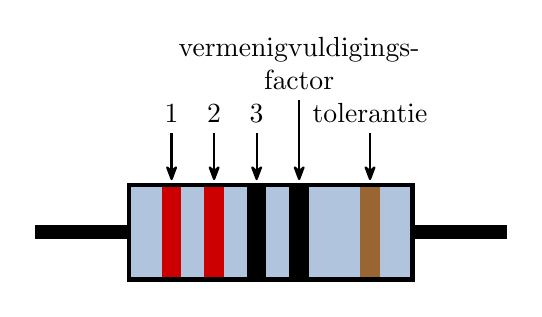
\begin{tikzpicture}[scale=.6]
\draw[line width=5pt] (0, 0) -- +(-2, 0) (6, 0) -- +(2, 0);
\fill[lightsteelblue] (0, -1) rectangle (6, 1);

\drawband{1}{Rred}{1}
\drawband{2}{Rred}{2}
\drawband{3}{black}{3}
\drawband[2em]{4}{black}{vermenigvuldigings-\\factor}
\drawband{5.1 / .9}{Rbrown}{tolerantie}

\draw[ultra thick] (0, -1) rectangle (6, 1);
\end{tikzpicture}
\end{document}